% Created by tikzDevice version 0.12.3.1 on 2023-04-24 12:26:55
% !TEX encoding = UTF-8 Unicode
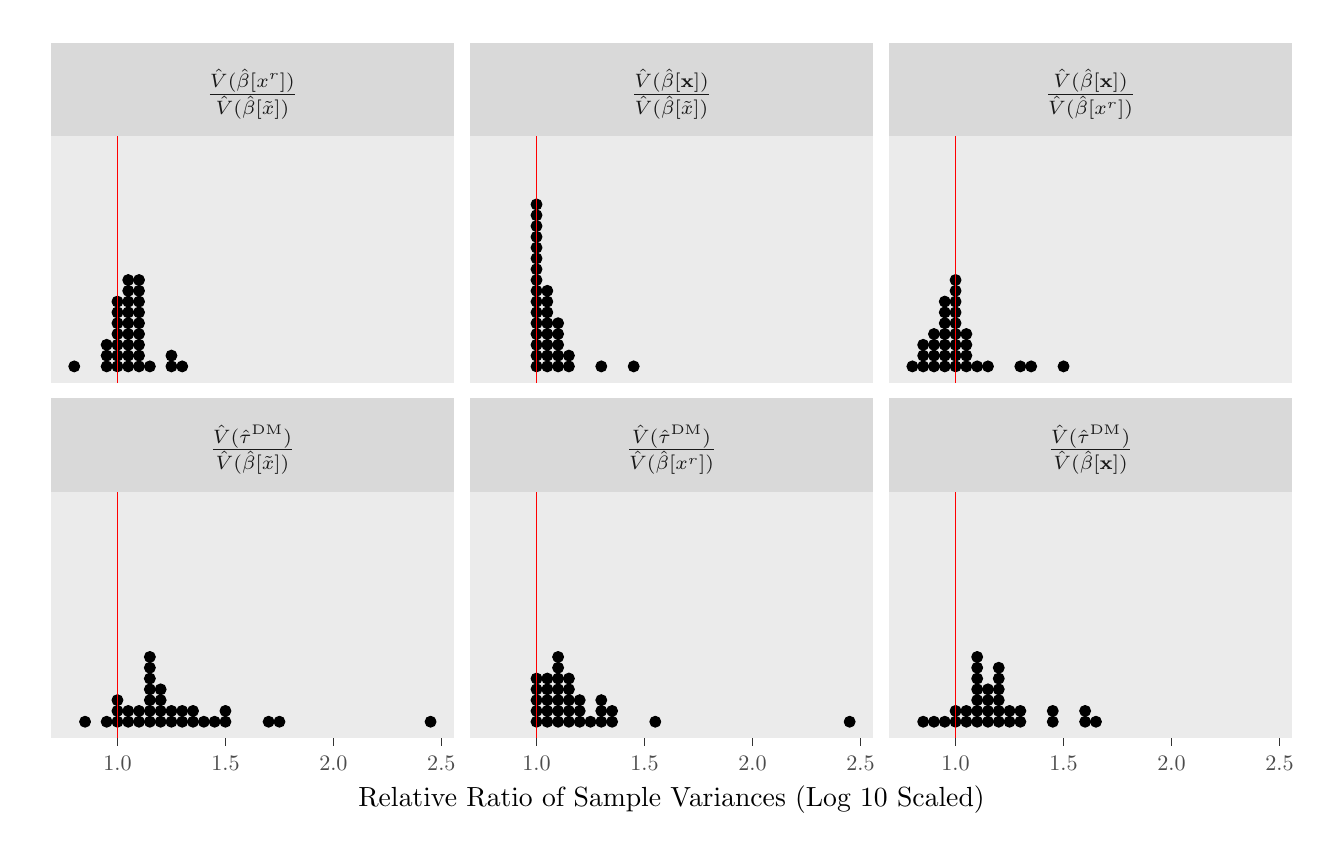
\begin{tikzpicture}[x=1pt,y=1pt]
\definecolor{fillColor}{RGB}{255,255,255}
\path[use as bounding box,fill=fillColor,fill opacity=0.00] (0,0) rectangle (462.53,289.08);
\begin{scope}
\path[clip] (  0.00,  0.00) rectangle (462.53,289.08);
\definecolor{drawColor}{RGB}{255,255,255}
\definecolor{fillColor}{RGB}{255,255,255}

\path[draw=drawColor,line width= 0.6pt,line join=round,line cap=round,fill=fillColor] (  0.00,  0.00) rectangle (462.53,289.08);
\end{scope}
\begin{scope}
\path[clip] (  8.25,160.68) rectangle (154.18,249.78);
\definecolor{fillColor}{gray}{0.92}

\path[fill=fillColor] (  8.25,160.68) rectangle (154.18,249.78);
\definecolor{drawColor}{RGB}{0,0,0}
\definecolor{fillColor}{RGB}{0,0,0}

\path[draw=drawColor,line width= 0.4pt,line join=round,fill=fillColor] ( 16.83,166.68) circle (  1.95);

\path[draw=drawColor,line width= 0.4pt,line join=round,fill=fillColor] ( 28.54,166.68) circle (  1.95);

\path[draw=drawColor,line width= 0.4pt,line join=round,fill=fillColor] ( 28.54,170.58) circle (  1.95);

\path[draw=drawColor,line width= 0.4pt,line join=round,fill=fillColor] ( 28.54,174.48) circle (  1.95);

\path[draw=drawColor,line width= 0.4pt,line join=round,fill=fillColor] ( 32.44,166.68) circle (  1.95);

\path[draw=drawColor,line width= 0.4pt,line join=round,fill=fillColor] ( 32.44,170.58) circle (  1.95);

\path[draw=drawColor,line width= 0.4pt,line join=round,fill=fillColor] ( 32.44,174.48) circle (  1.95);

\path[draw=drawColor,line width= 0.4pt,line join=round,fill=fillColor] ( 32.44,178.38) circle (  1.95);

\path[draw=drawColor,line width= 0.4pt,line join=round,fill=fillColor] ( 32.44,182.29) circle (  1.95);

\path[draw=drawColor,line width= 0.4pt,line join=round,fill=fillColor] ( 32.44,186.19) circle (  1.95);

\path[draw=drawColor,line width= 0.4pt,line join=round,fill=fillColor] ( 32.44,190.09) circle (  1.95);

\path[draw=drawColor,line width= 0.4pt,line join=round,fill=fillColor] ( 36.34,166.68) circle (  1.95);

\path[draw=drawColor,line width= 0.4pt,line join=round,fill=fillColor] ( 36.34,170.58) circle (  1.95);

\path[draw=drawColor,line width= 0.4pt,line join=round,fill=fillColor] ( 36.34,174.48) circle (  1.95);

\path[draw=drawColor,line width= 0.4pt,line join=round,fill=fillColor] ( 36.34,178.38) circle (  1.95);

\path[draw=drawColor,line width= 0.4pt,line join=round,fill=fillColor] ( 36.34,182.29) circle (  1.95);

\path[draw=drawColor,line width= 0.4pt,line join=round,fill=fillColor] ( 36.34,186.19) circle (  1.95);

\path[draw=drawColor,line width= 0.4pt,line join=round,fill=fillColor] ( 36.34,190.09) circle (  1.95);

\path[draw=drawColor,line width= 0.4pt,line join=round,fill=fillColor] ( 36.34,193.99) circle (  1.95);

\path[draw=drawColor,line width= 0.4pt,line join=round,fill=fillColor] ( 36.34,197.89) circle (  1.95);

\path[draw=drawColor,line width= 0.4pt,line join=round,fill=fillColor] ( 40.24,166.68) circle (  1.95);

\path[draw=drawColor,line width= 0.4pt,line join=round,fill=fillColor] ( 40.24,170.58) circle (  1.95);

\path[draw=drawColor,line width= 0.4pt,line join=round,fill=fillColor] ( 40.24,174.48) circle (  1.95);

\path[draw=drawColor,line width= 0.4pt,line join=round,fill=fillColor] ( 40.24,178.38) circle (  1.95);

\path[draw=drawColor,line width= 0.4pt,line join=round,fill=fillColor] ( 40.24,182.29) circle (  1.95);

\path[draw=drawColor,line width= 0.4pt,line join=round,fill=fillColor] ( 40.24,186.19) circle (  1.95);

\path[draw=drawColor,line width= 0.4pt,line join=round,fill=fillColor] ( 40.24,190.09) circle (  1.95);

\path[draw=drawColor,line width= 0.4pt,line join=round,fill=fillColor] ( 40.24,193.99) circle (  1.95);

\path[draw=drawColor,line width= 0.4pt,line join=round,fill=fillColor] ( 40.24,197.89) circle (  1.95);

\path[draw=drawColor,line width= 0.4pt,line join=round,fill=fillColor] ( 44.15,166.68) circle (  1.95);

\path[draw=drawColor,line width= 0.4pt,line join=round,fill=fillColor] ( 51.95,166.68) circle (  1.95);

\path[draw=drawColor,line width= 0.4pt,line join=round,fill=fillColor] ( 51.95,170.58) circle (  1.95);

\path[draw=drawColor,line width= 0.4pt,line join=round,fill=fillColor] ( 55.85,166.68) circle (  1.95);
\definecolor{drawColor}{RGB}{255,0,0}

\path[draw=drawColor,line width= 0.6pt,line join=round] ( 32.44,160.68) -- ( 32.44,249.78);
\end{scope}
\begin{scope}
\path[clip] (  8.25, 32.28) rectangle (154.18,121.38);
\definecolor{fillColor}{gray}{0.92}

\path[fill=fillColor] (  8.25, 32.28) rectangle (154.18,121.38);
\definecolor{drawColor}{RGB}{0,0,0}
\definecolor{fillColor}{RGB}{0,0,0}

\path[draw=drawColor,line width= 0.4pt,line join=round,fill=fillColor] ( 20.74, 38.28) circle (  1.95);

\path[draw=drawColor,line width= 0.4pt,line join=round,fill=fillColor] ( 28.54, 38.28) circle (  1.95);

\path[draw=drawColor,line width= 0.4pt,line join=round,fill=fillColor] ( 32.44, 38.28) circle (  1.95);

\path[draw=drawColor,line width= 0.4pt,line join=round,fill=fillColor] ( 32.44, 42.18) circle (  1.95);

\path[draw=drawColor,line width= 0.4pt,line join=round,fill=fillColor] ( 32.44, 46.08) circle (  1.95);

\path[draw=drawColor,line width= 0.4pt,line join=round,fill=fillColor] ( 36.34, 38.28) circle (  1.95);

\path[draw=drawColor,line width= 0.4pt,line join=round,fill=fillColor] ( 36.34, 42.18) circle (  1.95);

\path[draw=drawColor,line width= 0.4pt,line join=round,fill=fillColor] ( 40.24, 38.28) circle (  1.95);

\path[draw=drawColor,line width= 0.4pt,line join=round,fill=fillColor] ( 40.24, 42.18) circle (  1.95);

\path[draw=drawColor,line width= 0.4pt,line join=round,fill=fillColor] ( 44.15, 38.28) circle (  1.95);

\path[draw=drawColor,line width= 0.4pt,line join=round,fill=fillColor] ( 44.15, 42.18) circle (  1.95);

\path[draw=drawColor,line width= 0.4pt,line join=round,fill=fillColor] ( 44.15, 46.08) circle (  1.95);

\path[draw=drawColor,line width= 0.4pt,line join=round,fill=fillColor] ( 44.15, 49.98) circle (  1.95);

\path[draw=drawColor,line width= 0.4pt,line join=round,fill=fillColor] ( 44.15, 53.88) circle (  1.95);

\path[draw=drawColor,line width= 0.4pt,line join=round,fill=fillColor] ( 44.15, 57.79) circle (  1.95);

\path[draw=drawColor,line width= 0.4pt,line join=round,fill=fillColor] ( 44.15, 61.69) circle (  1.95);

\path[draw=drawColor,line width= 0.4pt,line join=round,fill=fillColor] ( 48.05, 38.28) circle (  1.95);

\path[draw=drawColor,line width= 0.4pt,line join=round,fill=fillColor] ( 48.05, 42.18) circle (  1.95);

\path[draw=drawColor,line width= 0.4pt,line join=round,fill=fillColor] ( 48.05, 46.08) circle (  1.95);

\path[draw=drawColor,line width= 0.4pt,line join=round,fill=fillColor] ( 48.05, 49.98) circle (  1.95);

\path[draw=drawColor,line width= 0.4pt,line join=round,fill=fillColor] ( 51.95, 38.28) circle (  1.95);

\path[draw=drawColor,line width= 0.4pt,line join=round,fill=fillColor] ( 51.95, 42.18) circle (  1.95);

\path[draw=drawColor,line width= 0.4pt,line join=round,fill=fillColor] ( 55.85, 38.28) circle (  1.95);

\path[draw=drawColor,line width= 0.4pt,line join=round,fill=fillColor] ( 55.85, 42.18) circle (  1.95);

\path[draw=drawColor,line width= 0.4pt,line join=round,fill=fillColor] ( 59.75, 38.28) circle (  1.95);

\path[draw=drawColor,line width= 0.4pt,line join=round,fill=fillColor] ( 59.75, 42.18) circle (  1.95);

\path[draw=drawColor,line width= 0.4pt,line join=round,fill=fillColor] ( 63.66, 38.28) circle (  1.95);

\path[draw=drawColor,line width= 0.4pt,line join=round,fill=fillColor] ( 67.56, 38.28) circle (  1.95);

\path[draw=drawColor,line width= 0.4pt,line join=round,fill=fillColor] ( 71.46, 38.28) circle (  1.95);

\path[draw=drawColor,line width= 0.4pt,line join=round,fill=fillColor] ( 71.46, 42.18) circle (  1.95);

\path[draw=drawColor,line width= 0.4pt,line join=round,fill=fillColor] ( 87.07, 38.28) circle (  1.95);

\path[draw=drawColor,line width= 0.4pt,line join=round,fill=fillColor] ( 90.97, 38.28) circle (  1.95);

\path[draw=drawColor,line width= 0.4pt,line join=round,fill=fillColor] (145.59, 38.28) circle (  1.95);
\definecolor{drawColor}{RGB}{255,0,0}

\path[draw=drawColor,line width= 0.6pt,line join=round] ( 32.44, 32.28) -- ( 32.44,121.38);
\end{scope}
\begin{scope}
\path[clip] (159.68,160.68) rectangle (305.60,249.78);
\definecolor{fillColor}{gray}{0.92}

\path[fill=fillColor] (159.68,160.68) rectangle (305.60,249.78);
\definecolor{drawColor}{RGB}{0,0,0}
\definecolor{fillColor}{RGB}{0,0,0}

\path[draw=drawColor,line width= 0.4pt,line join=round,fill=fillColor] (183.87,166.68) circle (  1.95);

\path[draw=drawColor,line width= 0.4pt,line join=round,fill=fillColor] (183.87,170.58) circle (  1.95);

\path[draw=drawColor,line width= 0.4pt,line join=round,fill=fillColor] (183.87,174.48) circle (  1.95);

\path[draw=drawColor,line width= 0.4pt,line join=round,fill=fillColor] (183.87,178.38) circle (  1.95);

\path[draw=drawColor,line width= 0.4pt,line join=round,fill=fillColor] (183.87,182.29) circle (  1.95);

\path[draw=drawColor,line width= 0.4pt,line join=round,fill=fillColor] (183.87,186.19) circle (  1.95);

\path[draw=drawColor,line width= 0.4pt,line join=round,fill=fillColor] (183.87,190.09) circle (  1.95);

\path[draw=drawColor,line width= 0.4pt,line join=round,fill=fillColor] (183.87,193.99) circle (  1.95);

\path[draw=drawColor,line width= 0.4pt,line join=round,fill=fillColor] (183.87,197.89) circle (  1.95);

\path[draw=drawColor,line width= 0.4pt,line join=round,fill=fillColor] (183.87,201.79) circle (  1.95);

\path[draw=drawColor,line width= 0.4pt,line join=round,fill=fillColor] (183.87,205.70) circle (  1.95);

\path[draw=drawColor,line width= 0.4pt,line join=round,fill=fillColor] (183.87,209.60) circle (  1.95);

\path[draw=drawColor,line width= 0.4pt,line join=round,fill=fillColor] (183.87,213.50) circle (  1.95);

\path[draw=drawColor,line width= 0.4pt,line join=round,fill=fillColor] (183.87,217.40) circle (  1.95);

\path[draw=drawColor,line width= 0.4pt,line join=round,fill=fillColor] (183.87,221.30) circle (  1.95);

\path[draw=drawColor,line width= 0.4pt,line join=round,fill=fillColor] (183.87,225.21) circle (  1.95);

\path[draw=drawColor,line width= 0.4pt,line join=round,fill=fillColor] (187.77,166.68) circle (  1.95);

\path[draw=drawColor,line width= 0.4pt,line join=round,fill=fillColor] (187.77,170.58) circle (  1.95);

\path[draw=drawColor,line width= 0.4pt,line join=round,fill=fillColor] (187.77,174.48) circle (  1.95);

\path[draw=drawColor,line width= 0.4pt,line join=round,fill=fillColor] (187.77,178.38) circle (  1.95);

\path[draw=drawColor,line width= 0.4pt,line join=round,fill=fillColor] (187.77,182.29) circle (  1.95);

\path[draw=drawColor,line width= 0.4pt,line join=round,fill=fillColor] (187.77,186.19) circle (  1.95);

\path[draw=drawColor,line width= 0.4pt,line join=round,fill=fillColor] (187.77,190.09) circle (  1.95);

\path[draw=drawColor,line width= 0.4pt,line join=round,fill=fillColor] (187.77,193.99) circle (  1.95);

\path[draw=drawColor,line width= 0.4pt,line join=round,fill=fillColor] (191.67,166.68) circle (  1.95);

\path[draw=drawColor,line width= 0.4pt,line join=round,fill=fillColor] (191.67,170.58) circle (  1.95);

\path[draw=drawColor,line width= 0.4pt,line join=round,fill=fillColor] (191.67,174.48) circle (  1.95);

\path[draw=drawColor,line width= 0.4pt,line join=round,fill=fillColor] (191.67,178.38) circle (  1.95);

\path[draw=drawColor,line width= 0.4pt,line join=round,fill=fillColor] (191.67,182.29) circle (  1.95);

\path[draw=drawColor,line width= 0.4pt,line join=round,fill=fillColor] (195.57,166.68) circle (  1.95);

\path[draw=drawColor,line width= 0.4pt,line join=round,fill=fillColor] (195.57,170.58) circle (  1.95);

\path[draw=drawColor,line width= 0.4pt,line join=round,fill=fillColor] (207.28,166.68) circle (  1.95);

\path[draw=drawColor,line width= 0.4pt,line join=round,fill=fillColor] (218.98,166.68) circle (  1.95);
\definecolor{drawColor}{RGB}{255,0,0}

\path[draw=drawColor,line width= 0.6pt,line join=round] (183.87,160.68) -- (183.87,249.78);
\end{scope}
\begin{scope}
\path[clip] (159.68, 32.28) rectangle (305.60,121.38);
\definecolor{fillColor}{gray}{0.92}

\path[fill=fillColor] (159.68, 32.28) rectangle (305.60,121.38);
\definecolor{drawColor}{RGB}{0,0,0}
\definecolor{fillColor}{RGB}{0,0,0}

\path[draw=drawColor,line width= 0.4pt,line join=round,fill=fillColor] (183.87, 38.28) circle (  1.95);

\path[draw=drawColor,line width= 0.4pt,line join=round,fill=fillColor] (183.87, 42.18) circle (  1.95);

\path[draw=drawColor,line width= 0.4pt,line join=round,fill=fillColor] (183.87, 46.08) circle (  1.95);

\path[draw=drawColor,line width= 0.4pt,line join=round,fill=fillColor] (183.87, 49.98) circle (  1.95);

\path[draw=drawColor,line width= 0.4pt,line join=round,fill=fillColor] (183.87, 53.88) circle (  1.95);

\path[draw=drawColor,line width= 0.4pt,line join=round,fill=fillColor] (187.77, 38.28) circle (  1.95);

\path[draw=drawColor,line width= 0.4pt,line join=round,fill=fillColor] (187.77, 42.18) circle (  1.95);

\path[draw=drawColor,line width= 0.4pt,line join=round,fill=fillColor] (187.77, 46.08) circle (  1.95);

\path[draw=drawColor,line width= 0.4pt,line join=round,fill=fillColor] (187.77, 49.98) circle (  1.95);

\path[draw=drawColor,line width= 0.4pt,line join=round,fill=fillColor] (187.77, 53.88) circle (  1.95);

\path[draw=drawColor,line width= 0.4pt,line join=round,fill=fillColor] (191.67, 38.28) circle (  1.95);

\path[draw=drawColor,line width= 0.4pt,line join=round,fill=fillColor] (191.67, 42.18) circle (  1.95);

\path[draw=drawColor,line width= 0.4pt,line join=round,fill=fillColor] (191.67, 46.08) circle (  1.95);

\path[draw=drawColor,line width= 0.4pt,line join=round,fill=fillColor] (191.67, 49.98) circle (  1.95);

\path[draw=drawColor,line width= 0.4pt,line join=round,fill=fillColor] (191.67, 53.88) circle (  1.95);

\path[draw=drawColor,line width= 0.4pt,line join=round,fill=fillColor] (191.67, 57.79) circle (  1.95);

\path[draw=drawColor,line width= 0.4pt,line join=round,fill=fillColor] (191.67, 61.69) circle (  1.95);

\path[draw=drawColor,line width= 0.4pt,line join=round,fill=fillColor] (195.57, 38.28) circle (  1.95);

\path[draw=drawColor,line width= 0.4pt,line join=round,fill=fillColor] (195.57, 42.18) circle (  1.95);

\path[draw=drawColor,line width= 0.4pt,line join=round,fill=fillColor] (195.57, 46.08) circle (  1.95);

\path[draw=drawColor,line width= 0.4pt,line join=round,fill=fillColor] (195.57, 49.98) circle (  1.95);

\path[draw=drawColor,line width= 0.4pt,line join=round,fill=fillColor] (195.57, 53.88) circle (  1.95);

\path[draw=drawColor,line width= 0.4pt,line join=round,fill=fillColor] (199.47, 38.28) circle (  1.95);

\path[draw=drawColor,line width= 0.4pt,line join=round,fill=fillColor] (199.47, 42.18) circle (  1.95);

\path[draw=drawColor,line width= 0.4pt,line join=round,fill=fillColor] (199.47, 46.08) circle (  1.95);

\path[draw=drawColor,line width= 0.4pt,line join=round,fill=fillColor] (203.38, 38.28) circle (  1.95);

\path[draw=drawColor,line width= 0.4pt,line join=round,fill=fillColor] (207.28, 38.28) circle (  1.95);

\path[draw=drawColor,line width= 0.4pt,line join=round,fill=fillColor] (207.28, 42.18) circle (  1.95);

\path[draw=drawColor,line width= 0.4pt,line join=round,fill=fillColor] (207.28, 46.08) circle (  1.95);

\path[draw=drawColor,line width= 0.4pt,line join=round,fill=fillColor] (211.18, 38.28) circle (  1.95);

\path[draw=drawColor,line width= 0.4pt,line join=round,fill=fillColor] (211.18, 42.18) circle (  1.95);

\path[draw=drawColor,line width= 0.4pt,line join=round,fill=fillColor] (226.79, 38.28) circle (  1.95);

\path[draw=drawColor,line width= 0.4pt,line join=round,fill=fillColor] (297.02, 38.28) circle (  1.95);
\definecolor{drawColor}{RGB}{255,0,0}

\path[draw=drawColor,line width= 0.6pt,line join=round] (183.87, 32.28) -- (183.87,121.38);
\end{scope}
\begin{scope}
\path[clip] (311.10,160.68) rectangle (457.03,249.78);
\definecolor{fillColor}{gray}{0.92}

\path[fill=fillColor] (311.10,160.68) rectangle (457.03,249.78);
\definecolor{drawColor}{RGB}{0,0,0}
\definecolor{fillColor}{RGB}{0,0,0}

\path[draw=drawColor,line width= 0.4pt,line join=round,fill=fillColor] (319.69,166.68) circle (  1.95);

\path[draw=drawColor,line width= 0.4pt,line join=round,fill=fillColor] (323.59,166.68) circle (  1.95);

\path[draw=drawColor,line width= 0.4pt,line join=round,fill=fillColor] (323.59,170.58) circle (  1.95);

\path[draw=drawColor,line width= 0.4pt,line join=round,fill=fillColor] (323.59,174.48) circle (  1.95);

\path[draw=drawColor,line width= 0.4pt,line join=round,fill=fillColor] (327.49,166.68) circle (  1.95);

\path[draw=drawColor,line width= 0.4pt,line join=round,fill=fillColor] (327.49,170.58) circle (  1.95);

\path[draw=drawColor,line width= 0.4pt,line join=round,fill=fillColor] (327.49,174.48) circle (  1.95);

\path[draw=drawColor,line width= 0.4pt,line join=round,fill=fillColor] (327.49,178.38) circle (  1.95);

\path[draw=drawColor,line width= 0.4pt,line join=round,fill=fillColor] (331.39,166.68) circle (  1.95);

\path[draw=drawColor,line width= 0.4pt,line join=round,fill=fillColor] (331.39,170.58) circle (  1.95);

\path[draw=drawColor,line width= 0.4pt,line join=round,fill=fillColor] (331.39,174.48) circle (  1.95);

\path[draw=drawColor,line width= 0.4pt,line join=round,fill=fillColor] (331.39,178.38) circle (  1.95);

\path[draw=drawColor,line width= 0.4pt,line join=round,fill=fillColor] (331.39,182.29) circle (  1.95);

\path[draw=drawColor,line width= 0.4pt,line join=round,fill=fillColor] (331.39,186.19) circle (  1.95);

\path[draw=drawColor,line width= 0.4pt,line join=round,fill=fillColor] (331.39,190.09) circle (  1.95);

\path[draw=drawColor,line width= 0.4pt,line join=round,fill=fillColor] (335.29,166.68) circle (  1.95);

\path[draw=drawColor,line width= 0.4pt,line join=round,fill=fillColor] (335.29,170.58) circle (  1.95);

\path[draw=drawColor,line width= 0.4pt,line join=round,fill=fillColor] (335.29,174.48) circle (  1.95);

\path[draw=drawColor,line width= 0.4pt,line join=round,fill=fillColor] (335.29,178.38) circle (  1.95);

\path[draw=drawColor,line width= 0.4pt,line join=round,fill=fillColor] (335.29,182.29) circle (  1.95);

\path[draw=drawColor,line width= 0.4pt,line join=round,fill=fillColor] (335.29,186.19) circle (  1.95);

\path[draw=drawColor,line width= 0.4pt,line join=round,fill=fillColor] (335.29,190.09) circle (  1.95);

\path[draw=drawColor,line width= 0.4pt,line join=round,fill=fillColor] (335.29,193.99) circle (  1.95);

\path[draw=drawColor,line width= 0.4pt,line join=round,fill=fillColor] (335.29,197.89) circle (  1.95);

\path[draw=drawColor,line width= 0.4pt,line join=round,fill=fillColor] (339.19,166.68) circle (  1.95);

\path[draw=drawColor,line width= 0.4pt,line join=round,fill=fillColor] (339.19,170.58) circle (  1.95);

\path[draw=drawColor,line width= 0.4pt,line join=round,fill=fillColor] (339.19,174.48) circle (  1.95);

\path[draw=drawColor,line width= 0.4pt,line join=round,fill=fillColor] (339.19,178.38) circle (  1.95);

\path[draw=drawColor,line width= 0.4pt,line join=round,fill=fillColor] (343.10,166.68) circle (  1.95);

\path[draw=drawColor,line width= 0.4pt,line join=round,fill=fillColor] (347.00,166.68) circle (  1.95);

\path[draw=drawColor,line width= 0.4pt,line join=round,fill=fillColor] (358.70,166.68) circle (  1.95);

\path[draw=drawColor,line width= 0.4pt,line join=round,fill=fillColor] (362.61,166.68) circle (  1.95);

\path[draw=drawColor,line width= 0.4pt,line join=round,fill=fillColor] (374.31,166.68) circle (  1.95);
\definecolor{drawColor}{RGB}{255,0,0}

\path[draw=drawColor,line width= 0.6pt,line join=round] (335.29,160.68) -- (335.29,249.78);
\end{scope}
\begin{scope}
\path[clip] (311.10, 32.28) rectangle (457.03,121.38);
\definecolor{fillColor}{gray}{0.92}

\path[fill=fillColor] (311.10, 32.28) rectangle (457.03,121.38);
\definecolor{drawColor}{RGB}{0,0,0}
\definecolor{fillColor}{RGB}{0,0,0}

\path[draw=drawColor,line width= 0.4pt,line join=round,fill=fillColor] (323.59, 38.28) circle (  1.95);

\path[draw=drawColor,line width= 0.4pt,line join=round,fill=fillColor] (327.49, 38.28) circle (  1.95);

\path[draw=drawColor,line width= 0.4pt,line join=round,fill=fillColor] (331.39, 38.28) circle (  1.95);

\path[draw=drawColor,line width= 0.4pt,line join=round,fill=fillColor] (335.29, 38.28) circle (  1.95);

\path[draw=drawColor,line width= 0.4pt,line join=round,fill=fillColor] (335.29, 42.18) circle (  1.95);

\path[draw=drawColor,line width= 0.4pt,line join=round,fill=fillColor] (339.19, 38.28) circle (  1.95);

\path[draw=drawColor,line width= 0.4pt,line join=round,fill=fillColor] (339.19, 42.18) circle (  1.95);

\path[draw=drawColor,line width= 0.4pt,line join=round,fill=fillColor] (343.10, 38.28) circle (  1.95);

\path[draw=drawColor,line width= 0.4pt,line join=round,fill=fillColor] (343.10, 42.18) circle (  1.95);

\path[draw=drawColor,line width= 0.4pt,line join=round,fill=fillColor] (343.10, 46.08) circle (  1.95);

\path[draw=drawColor,line width= 0.4pt,line join=round,fill=fillColor] (343.10, 49.98) circle (  1.95);

\path[draw=drawColor,line width= 0.4pt,line join=round,fill=fillColor] (343.10, 53.88) circle (  1.95);

\path[draw=drawColor,line width= 0.4pt,line join=round,fill=fillColor] (343.10, 57.79) circle (  1.95);

\path[draw=drawColor,line width= 0.4pt,line join=round,fill=fillColor] (343.10, 61.69) circle (  1.95);

\path[draw=drawColor,line width= 0.4pt,line join=round,fill=fillColor] (347.00, 38.28) circle (  1.95);

\path[draw=drawColor,line width= 0.4pt,line join=round,fill=fillColor] (347.00, 42.18) circle (  1.95);

\path[draw=drawColor,line width= 0.4pt,line join=round,fill=fillColor] (347.00, 46.08) circle (  1.95);

\path[draw=drawColor,line width= 0.4pt,line join=round,fill=fillColor] (347.00, 49.98) circle (  1.95);

\path[draw=drawColor,line width= 0.4pt,line join=round,fill=fillColor] (350.90, 38.28) circle (  1.95);

\path[draw=drawColor,line width= 0.4pt,line join=round,fill=fillColor] (350.90, 42.18) circle (  1.95);

\path[draw=drawColor,line width= 0.4pt,line join=round,fill=fillColor] (350.90, 46.08) circle (  1.95);

\path[draw=drawColor,line width= 0.4pt,line join=round,fill=fillColor] (350.90, 49.98) circle (  1.95);

\path[draw=drawColor,line width= 0.4pt,line join=round,fill=fillColor] (350.90, 53.88) circle (  1.95);

\path[draw=drawColor,line width= 0.4pt,line join=round,fill=fillColor] (350.90, 57.79) circle (  1.95);

\path[draw=drawColor,line width= 0.4pt,line join=round,fill=fillColor] (354.80, 38.28) circle (  1.95);

\path[draw=drawColor,line width= 0.4pt,line join=round,fill=fillColor] (354.80, 42.18) circle (  1.95);

\path[draw=drawColor,line width= 0.4pt,line join=round,fill=fillColor] (358.70, 38.28) circle (  1.95);

\path[draw=drawColor,line width= 0.4pt,line join=round,fill=fillColor] (358.70, 42.18) circle (  1.95);

\path[draw=drawColor,line width= 0.4pt,line join=round,fill=fillColor] (370.41, 38.28) circle (  1.95);

\path[draw=drawColor,line width= 0.4pt,line join=round,fill=fillColor] (370.41, 42.18) circle (  1.95);

\path[draw=drawColor,line width= 0.4pt,line join=round,fill=fillColor] (382.11, 38.28) circle (  1.95);

\path[draw=drawColor,line width= 0.4pt,line join=round,fill=fillColor] (382.11, 42.18) circle (  1.95);

\path[draw=drawColor,line width= 0.4pt,line join=round,fill=fillColor] (386.02, 38.28) circle (  1.95);
\definecolor{drawColor}{RGB}{255,0,0}

\path[draw=drawColor,line width= 0.6pt,line join=round] (335.29, 32.28) -- (335.29,121.38);
\end{scope}
\begin{scope}
\path[clip] (  8.25,121.38) rectangle (154.18,155.18);
\definecolor{fillColor}{gray}{0.85}

\path[fill=fillColor] (  8.25,121.38) rectangle (154.18,155.18);
\definecolor{drawColor}{gray}{0.10}

\node[text=drawColor,anchor=base,inner sep=0pt, outer sep=0pt, scale=  1.00] at ( 81.21,141.35) {};

\node[text=drawColor,anchor=base,inner sep=0pt, outer sep=0pt, scale=  1.00] at ( 81.21,134.15) {$\frac{\hat{\mathbb{V}}(\hat{\tau}^{\mathrm{DM}})}{\hat{\mathbb{V}}(\hat{\beta}[\tilde{x}])}$};

\node[text=drawColor,anchor=base,inner sep=0pt, outer sep=0pt, scale=  1.00] at ( 81.21,126.95) {};
\end{scope}
\begin{scope}
\path[clip] (159.68,121.38) rectangle (305.60,155.18);
\definecolor{fillColor}{gray}{0.85}

\path[fill=fillColor] (159.68,121.38) rectangle (305.60,155.18);
\definecolor{drawColor}{gray}{0.10}

\node[text=drawColor,anchor=base,inner sep=0pt, outer sep=0pt, scale=  1.00] at (232.64,141.35) {};

\node[text=drawColor,anchor=base,inner sep=0pt, outer sep=0pt, scale=  1.00] at (232.64,134.15) {$\frac{\hat{\mathbb{V}}(\hat{\tau}^{\mathrm{DM}})}{\hat{\mathbb{V}}(\hat{\beta}[x^r])}$};

\node[text=drawColor,anchor=base,inner sep=0pt, outer sep=0pt, scale=  1.00] at (232.64,126.95) {};
\end{scope}
\begin{scope}
\path[clip] (311.10,121.38) rectangle (457.03,155.18);
\definecolor{fillColor}{gray}{0.85}

\path[fill=fillColor] (311.10,121.38) rectangle (457.03,155.18);
\definecolor{drawColor}{gray}{0.10}

\node[text=drawColor,anchor=base,inner sep=0pt, outer sep=0pt, scale=  1.00] at (384.06,141.35) {};

\node[text=drawColor,anchor=base,inner sep=0pt, outer sep=0pt, scale=  1.00] at (384.06,134.15) {$\frac{\hat{\mathbb{V}}(\hat{\tau}^{\mathrm{DM}})}{\hat{\mathbb{V}}(\hat{\beta}[\mathbf{x}])}$};

\node[text=drawColor,anchor=base,inner sep=0pt, outer sep=0pt, scale=  1.00] at (384.06,126.95) {};
\end{scope}
\begin{scope}
\path[clip] (  8.25,249.78) rectangle (154.18,283.58);
\definecolor{fillColor}{gray}{0.85}

\path[fill=fillColor] (  8.25,249.78) rectangle (154.18,283.58);
\definecolor{drawColor}{gray}{0.10}

\node[text=drawColor,anchor=base,inner sep=0pt, outer sep=0pt, scale=  1.00] at ( 81.21,269.75) {};

\node[text=drawColor,anchor=base,inner sep=0pt, outer sep=0pt, scale=  1.00] at ( 81.21,262.55) {$\frac{\hat{\mathbb{V}}(\hat{\beta}[x^r])}{\hat{\mathbb{V}}(\hat{\beta}[\tilde{x}])}$};

\node[text=drawColor,anchor=base,inner sep=0pt, outer sep=0pt, scale=  1.00] at ( 81.21,255.35) {};
\end{scope}
\begin{scope}
\path[clip] (159.68,249.78) rectangle (305.60,283.58);
\definecolor{fillColor}{gray}{0.85}

\path[fill=fillColor] (159.68,249.78) rectangle (305.60,283.58);
\definecolor{drawColor}{gray}{0.10}

\node[text=drawColor,anchor=base,inner sep=0pt, outer sep=0pt, scale=  1.00] at (232.64,269.75) {};

\node[text=drawColor,anchor=base,inner sep=0pt, outer sep=0pt, scale=  1.00] at (232.64,262.55) {$\frac{\hat{\mathbb{V}}(\hat{\beta}[\mathbf{x}])}{\hat{\mathbb{V}}(\hat{\beta}[\tilde{x}])}$};

\node[text=drawColor,anchor=base,inner sep=0pt, outer sep=0pt, scale=  1.00] at (232.64,255.35) {};
\end{scope}
\begin{scope}
\path[clip] (311.10,249.78) rectangle (457.03,283.58);
\definecolor{fillColor}{gray}{0.85}

\path[fill=fillColor] (311.10,249.78) rectangle (457.03,283.58);
\definecolor{drawColor}{gray}{0.10}

\node[text=drawColor,anchor=base,inner sep=0pt, outer sep=0pt, scale=  1.00] at (384.06,269.75) {};

\node[text=drawColor,anchor=base,inner sep=0pt, outer sep=0pt, scale=  1.00] at (384.06,262.55) {$\frac{\hat{\mathbb{V}}(\hat{\beta}[\mathbf{x}])}{\hat{\mathbb{V}}(\hat{\beta}[x^r])}$};

\node[text=drawColor,anchor=base,inner sep=0pt, outer sep=0pt, scale=  1.00] at (384.06,255.35) {};
\end{scope}
\begin{scope}
\path[clip] (  0.00,  0.00) rectangle (462.53,289.08);
\definecolor{drawColor}{gray}{0.20}

\path[draw=drawColor,line width= 0.6pt,line join=round] ( 32.44, 29.53) --
	( 32.44, 32.28);

\path[draw=drawColor,line width= 0.6pt,line join=round] ( 71.46, 29.53) --
	( 71.46, 32.28);

\path[draw=drawColor,line width= 0.6pt,line join=round] (110.48, 29.53) --
	(110.48, 32.28);

\path[draw=drawColor,line width= 0.6pt,line join=round] (149.49, 29.53) --
	(149.49, 32.28);
\end{scope}
\begin{scope}
\path[clip] (  0.00,  0.00) rectangle (462.53,289.08);
\definecolor{drawColor}{gray}{0.30}

\node[text=drawColor,anchor=base,inner sep=0pt, outer sep=0pt, scale=  0.80] at ( 32.44, 20.71) {1.0};

\node[text=drawColor,anchor=base,inner sep=0pt, outer sep=0pt, scale=  0.80] at ( 71.46, 20.71) {1.5};

\node[text=drawColor,anchor=base,inner sep=0pt, outer sep=0pt, scale=  0.80] at (110.48, 20.71) {2.0};

\node[text=drawColor,anchor=base,inner sep=0pt, outer sep=0pt, scale=  0.80] at (149.49, 20.71) {2.5};
\end{scope}
\begin{scope}
\path[clip] (  0.00,  0.00) rectangle (462.53,289.08);
\definecolor{drawColor}{gray}{0.20}

\path[draw=drawColor,line width= 0.6pt,line join=round] (183.87, 29.53) --
	(183.87, 32.28);

\path[draw=drawColor,line width= 0.6pt,line join=round] (222.88, 29.53) --
	(222.88, 32.28);

\path[draw=drawColor,line width= 0.6pt,line join=round] (261.90, 29.53) --
	(261.90, 32.28);

\path[draw=drawColor,line width= 0.6pt,line join=round] (300.92, 29.53) --
	(300.92, 32.28);
\end{scope}
\begin{scope}
\path[clip] (  0.00,  0.00) rectangle (462.53,289.08);
\definecolor{drawColor}{gray}{0.30}

\node[text=drawColor,anchor=base,inner sep=0pt, outer sep=0pt, scale=  0.80] at (183.87, 20.71) {1.0};

\node[text=drawColor,anchor=base,inner sep=0pt, outer sep=0pt, scale=  0.80] at (222.88, 20.71) {1.5};

\node[text=drawColor,anchor=base,inner sep=0pt, outer sep=0pt, scale=  0.80] at (261.90, 20.71) {2.0};

\node[text=drawColor,anchor=base,inner sep=0pt, outer sep=0pt, scale=  0.80] at (300.92, 20.71) {2.5};
\end{scope}
\begin{scope}
\path[clip] (  0.00,  0.00) rectangle (462.53,289.08);
\definecolor{drawColor}{gray}{0.20}

\path[draw=drawColor,line width= 0.6pt,line join=round] (335.29, 29.53) --
	(335.29, 32.28);

\path[draw=drawColor,line width= 0.6pt,line join=round] (374.31, 29.53) --
	(374.31, 32.28);

\path[draw=drawColor,line width= 0.6pt,line join=round] (413.33, 29.53) --
	(413.33, 32.28);

\path[draw=drawColor,line width= 0.6pt,line join=round] (452.35, 29.53) --
	(452.35, 32.28);
\end{scope}
\begin{scope}
\path[clip] (  0.00,  0.00) rectangle (462.53,289.08);
\definecolor{drawColor}{gray}{0.30}

\node[text=drawColor,anchor=base,inner sep=0pt, outer sep=0pt, scale=  0.80] at (335.29, 20.71) {1.0};

\node[text=drawColor,anchor=base,inner sep=0pt, outer sep=0pt, scale=  0.80] at (374.31, 20.71) {1.5};

\node[text=drawColor,anchor=base,inner sep=0pt, outer sep=0pt, scale=  0.80] at (413.33, 20.71) {2.0};

\node[text=drawColor,anchor=base,inner sep=0pt, outer sep=0pt, scale=  0.80] at (452.35, 20.71) {2.5};
\end{scope}
\begin{scope}
\path[clip] (  0.00,  0.00) rectangle (462.53,289.08);
\definecolor{drawColor}{RGB}{0,0,0}

\node[text=drawColor,anchor=base,inner sep=0pt, outer sep=0pt, scale=  1.00] at (232.64,  7.83) {Relative Ratio of Sample Variances (Log 10 Scaled)};
\end{scope}
\end{tikzpicture}
